\chapter{Metodologia}
\label{c.metodologia}

%   ---------------------   EDITAR PARA O QUE REALMENTE ACONTECEU -------------------

Inicialmente, será elaborado o documento GDD e o projeto de arquitetura de software, que contribuem para a organização da estrutura, roteiro, cenários e personagens do jogo. Isso será feito de forma paralela com um levantamento bibliográfico mais aprofundado sobre saúde mental, traumas, problemas emocionais, distúrbios mentais e mecanismos de enfrentamento saudáveis.

Depois que os documentos forem elaborados, será iniciado o desenvolvimento do jogo, desenhando o ambiente de cada cena e programando cada mecânica. Quando o levantamento bibliográfico sobre saúde mental for concluído, uma pesquisa sobre modelos de IA para animação será feita, analisando quais as técnicas utilizadas por cada um, as vantagens, as desvantagens e o foco. Após a pesquisa, será escolhido um modelo para ser treinado, implementado e modificado conforme necessário. O treinamento será feito de forma paralela com o desenvolvimento do jogo. Após a IA ter sido treinada, ela será utilizada para fazer as animações dos personagens do jogo. Durante o estudo, treinamento e implementação do modelo da IA, será feita uma análise de como o modelo ajuda no cenário de animações 2D, documentando qualquer modificação feita. Ao longo do desenvolvimento, serão realizados diversos testes para verificar se o comportamento está de acordo com o esperado. 

A partir do momento em que o jogo for concluído, serão realizados testes finais para verificar o funcionamento correto de todos os elementos, fazendo ajustes se necessário. O planejamento da ordem em que cada atividade será realizada é demonstrado pela Figura \ref{f.Diagrama}.

\begin{figure}[htbp]
	\caption{\small Fluxograma das etapas}
	\centering
	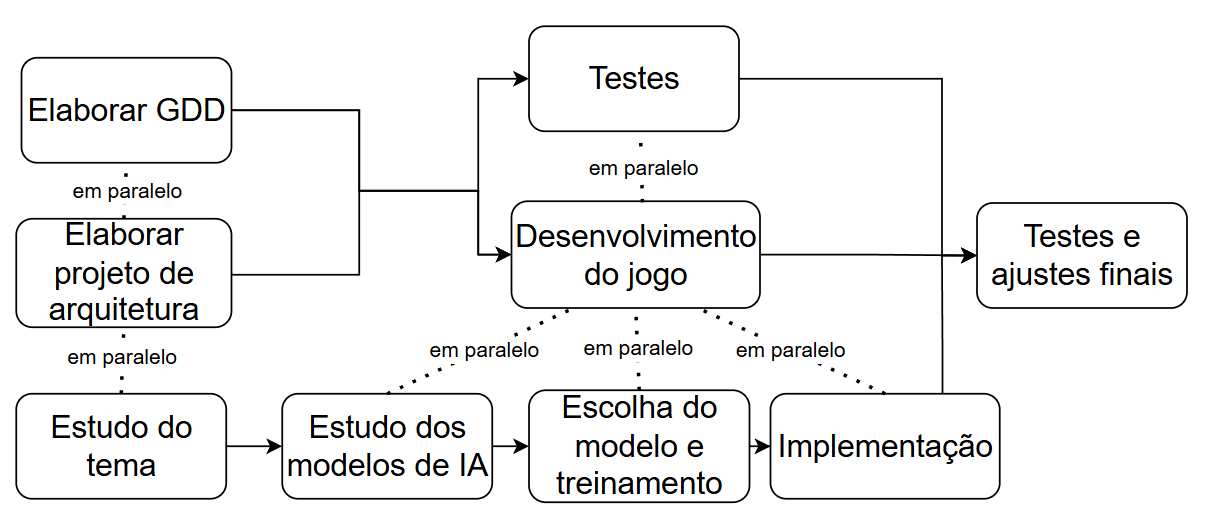
\includegraphics[width=1\linewidth]{figs/Diagrama.PNG}
	\label{f.Diagrama}
	\legend{\small Fonte: Elaborada pela autora.}
\end{figure}

%   ------------------------------------------------------------------------
\FloatBarrier
\section{Metodologia de desenvolvimento do jogo}
\label{s.jogo}

\FloatBarrier
\section{Metodologia de Análise das Ferramentas de IA}
\label{s.ia}


Para conduzir a análise comparativa das ferramentas de IA, a metodologia foi estruturada em etapas, partindo de uma seleção ampla de ferramentas até uma avaliação aprofundada das mais promissoras.

Inicialmente, foram estabelecidos os seguintes critérios de seleção para a escolha de ferramentas:

\begin{itemize}
\item Capacidade de criar vídeos ou imagens que pudessem ser usados para a animação 2D;
\item Disponibilidade de um modelo de acesso gratuito, ainda que com limitações de uso;
\item Possibilidade de usar uma imagem pré-existente (do personagem ou objeto) como referência, para consistência visual; e
\item Acessível para um usuário sem conhecimento aprofundado na ferramenta.
\end{itemize}

%------------------------ CHECAR SE NÃO OLHOU NENHUMA NOVA NÃO MENCIONADA ----------------
Com base nesses critérios, foram selecionados os seguintes softwares como candidatos para a produção de animação 2D: CGDream \cite{cgdream_2025}, ChatGPT \cite{chatgpt_2025}, OpenArtAI\cite{openArtai_2025}, geminiPro \cite{gemini_2025}, God Mode AI \cite{godmodeanimation2024}, PixelLab \cite{pixelLab}, PixieHaus \cite{pixie.haus_2025}, Rosebud AI \cite{rosebud}, Animated Drawings \cite{animatedDrawings}, Vidu \cite{viduai_2024}, AI Sprite Sheet Maker \cite{segmind} e SpriteSheetGPT \cite{spritesheetgpt-free}. 


O processo de análise foi dividido em duas fases. A primeira fase consistiu em uma análise geral de cada ferramenta, verificando os recursos grátis disponíveis, as opções de customização existentes e a capacidade de gerar uma animação 2D útil para o jogo em desenvolvimento a partir de um sprite de referência. Essa triagem inicial permitiu descartar algumas ferramentas que provaram não ser capazes de alcançar o resultado desejado, sobrando apenas as candidatas mais promissoras. Um desafio descoberto nesta etapa foi a limitação de uso do modelo gratuito de muitas plataformas, o que restringiu o número de testes comparativos e reduziu o número de gerações.

Na segunda fase, foi realizado um aprofundamento das ferramentas restantes. Foram conduzidos testes iterativos com diversos prompts (a maioria em inglês para melhores resultados) e imagens de referências nas plataformas que não possuíam um limite para o uso gratuito, ou este era muito alto. Para as plataformas mais restritas, os resultados que chegavam mais perto do desejado eram usados como referência para os outros softwares. As animações satisfatórias foram implementadas no jogo, com o uso de ferramentas auxiliares para converter ou ajustar o formato do arquivo e para pequenas edições na imagem.

%------------- CHECAR SE NÃO CRIOU NENHUMA ANIMAÇÃO NOVA NÃO MENCIONADA ----------------
Foram criadas animações com IA para alguns elementos do jogo: o personagem Pablo (Figura \ref{fig:Pablo}), que realiza as ações de andar, pular, virar de costas e sentar; a personagem Luz; e a porta (Figuras \ref{fig:portaA}, \ref{fig:portaB}) e \ref{fig:portaC}, que executa os movimentos de abrir e fechar. Os resultados adequados foram implementados no jogo.


\begin{figure}[htbp]
    \centering
    \caption{\small Sprite do Pablo}
    
\includegraphics[width=0.3\linewidth]{figs/sprites/Pablo.PNG}
    \label{fig:Pablo}
    \legend{\small Fonte: Elaborada pela autora.}
\end{figure}


\begin{figure}[htbp]
    \centering
    \caption{\small Sprite da Luz}
    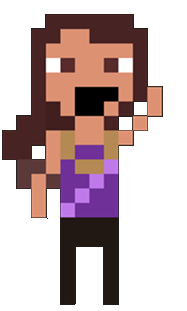
\includegraphics[width=0.3\linewidth]{figs/sprites/irma.PNG}
    \label{fig:Luz}
    \legend{\small Fonte: Elaborada pela autora.}
\end{figure}


\begin{figure}[htbp]
    \centering
    \begin{minipage}{0.45\textwidth}
    \caption{\small Sprite da porta A em front view (vista frontal, em inglês)}
    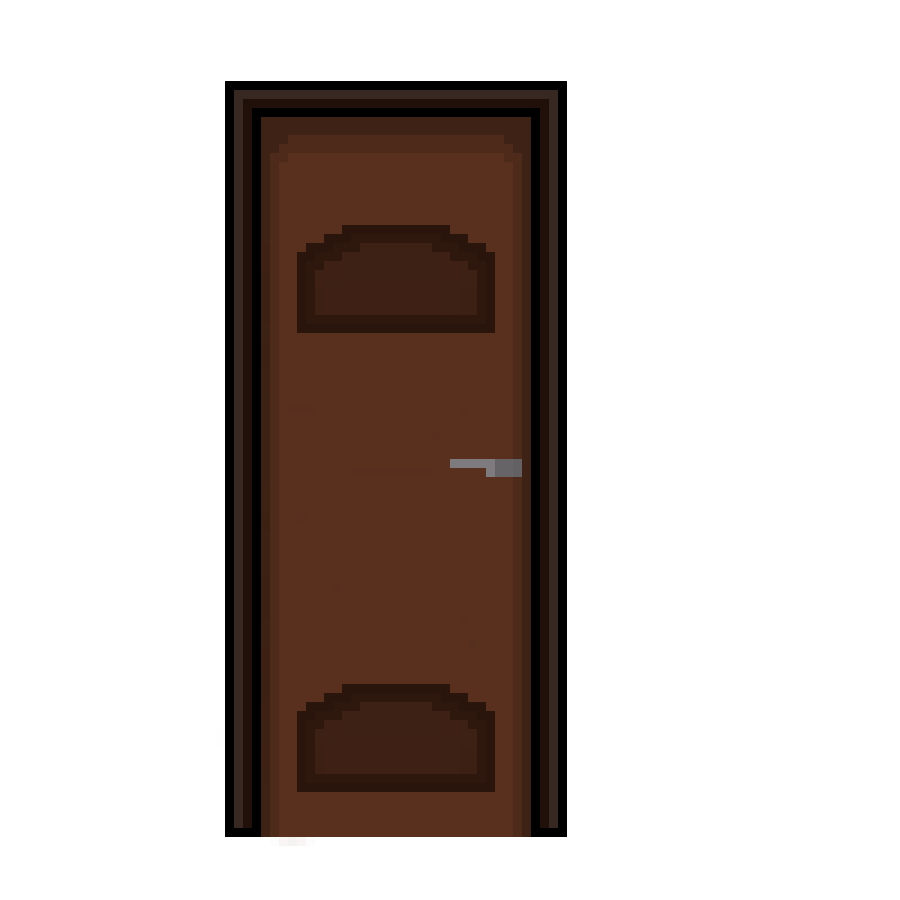
\includegraphics[width=1\linewidth]{figs/sprites/Porta front view.png}
    \label{fig:portaA}
    \legend{\small Fonte: Elaborada pela autora.}
    \end{minipage}\hfill
    \begin{minipage}{0.45\textwidth}
    \caption{\small Sprite da porta B em side view (vista lateral, em inglês)}
    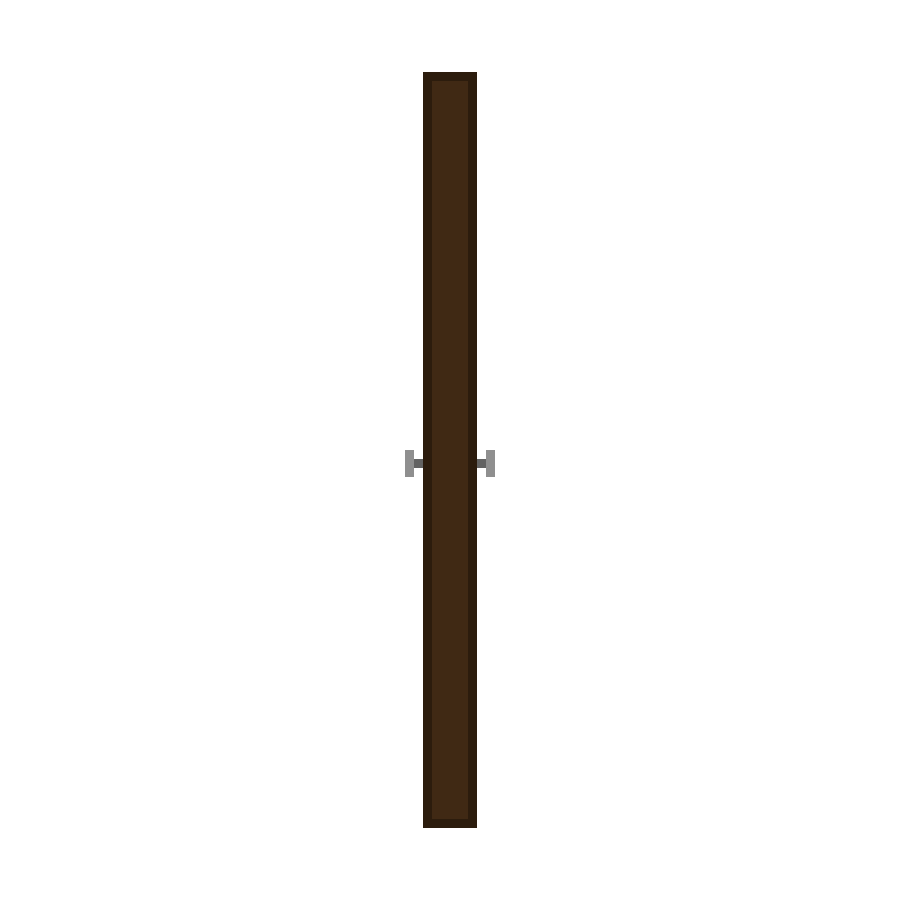
\includegraphics[width=1\linewidth]{figs/sprites/Porta side view.png}
    \label{fig:portaB}
    \legend{\small Fonte: Elaborada pela autora.}
    \end{minipage}\hfill
\end{figure}


\begin{figure}[htbp]
    \centering
    \caption{\small Sprites da porta C}
    \label{fig:portaC}
    \begin{subfigure}{0.45\textwidth}
    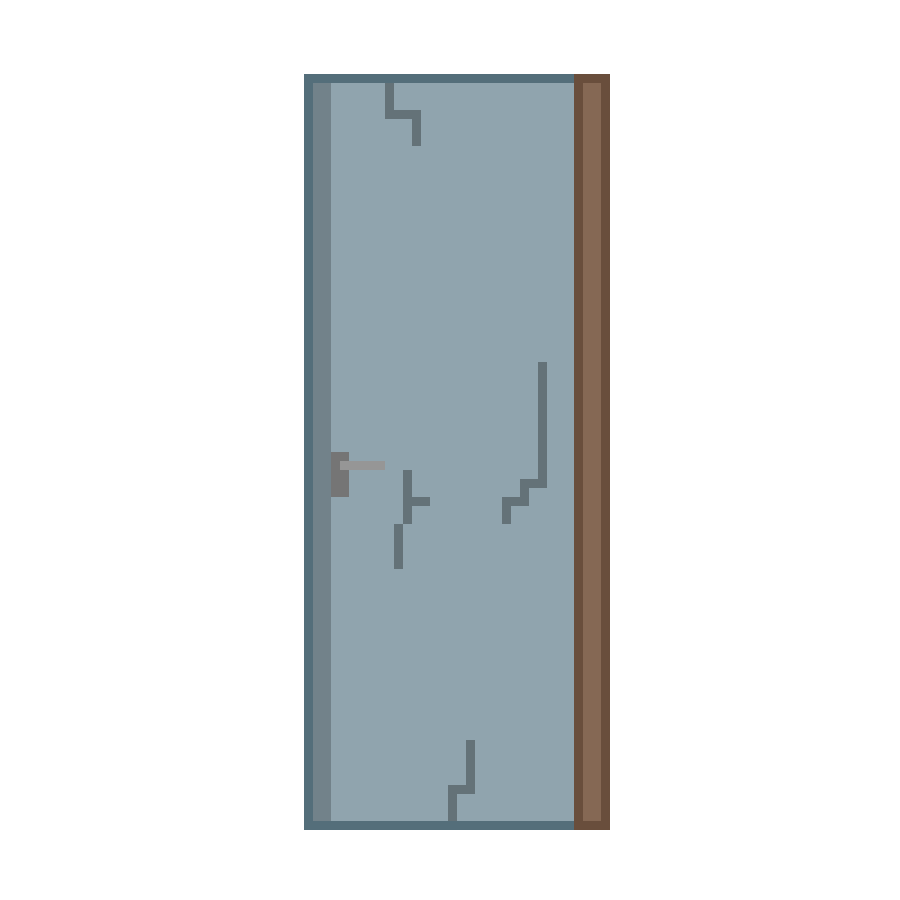
\includegraphics[width=1\linewidth]{figs/sprites/referencia_porta_tutorial (1).png}
    \caption{\small Sprite da porta C aberta em side view}
    \label{fig:portaCAberto}
    \end{subfigure}\hfill
    \begin{subfigure}{0.45\textwidth}
    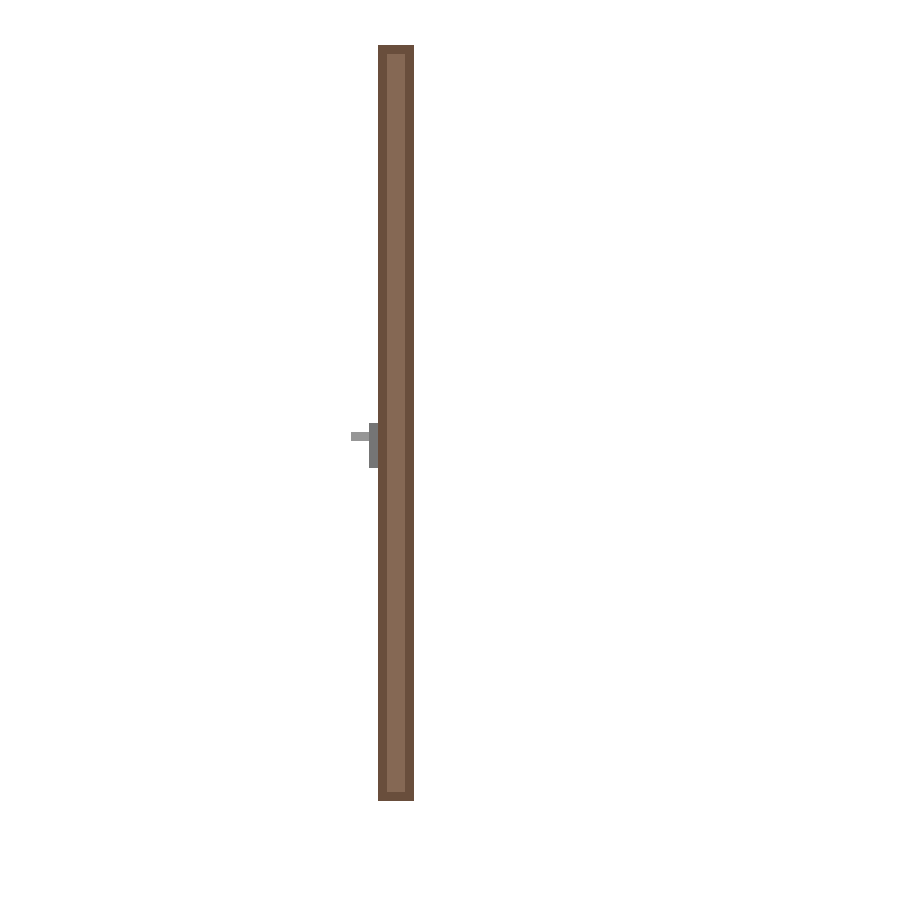
\includegraphics[width=1\linewidth]{figs/sprites/referencia_porta_tutorial (2).png}
    \caption{\small Sprite da porta C fechada em side view}
    \label{fig:portaCFechado}

    \end{subfigure}\hfill
    \legend{\small Fonte: Elaborada pela autora.}
\end{figure}

Ao final do processo, as ferramentas mais satisfatórias serão comparadas e avaliadas pelos seguintes critérios:

\begin{itemize}
\item Foco em 2D;
\item Consistência com o estilo e cores da imagem de referência;
\item Facilidade de uso e curva de aprendizagem;
\item Precisão de movimento e fidelidade ao prompt;
\item Qualidade estética;
\item Nível de customização;
\item Eficiência;
\item Capacidade de produzir resultado pixel perfect (todos os pixels tem o mesmo tamanho); e
\item Capacidade de edição e refinamento do material gerado.
\end{itemize}
